\documentclass[border=10pt]{standalone}
\usepackage[T1]{fontenc}
\usepackage{helvet}
\renewcommand{\familydefault}{\sfdefault}
\usepackage{tikz}
\usetikzlibrary{arrows.meta,positioning,calc,backgrounds}

\definecolor{idpblue}{HTML}{005DAA}
\definecolor{idpcyan}{HTML}{00B3FF}
\definecolor{warm}{HTML}{D7263D}
\definecolor{amber}{HTML}{E08A00}
\definecolor{inkgray}{HTML}{444444}
\definecolor{forestgreen}{HTML}{2E7D32}

\begin{document}
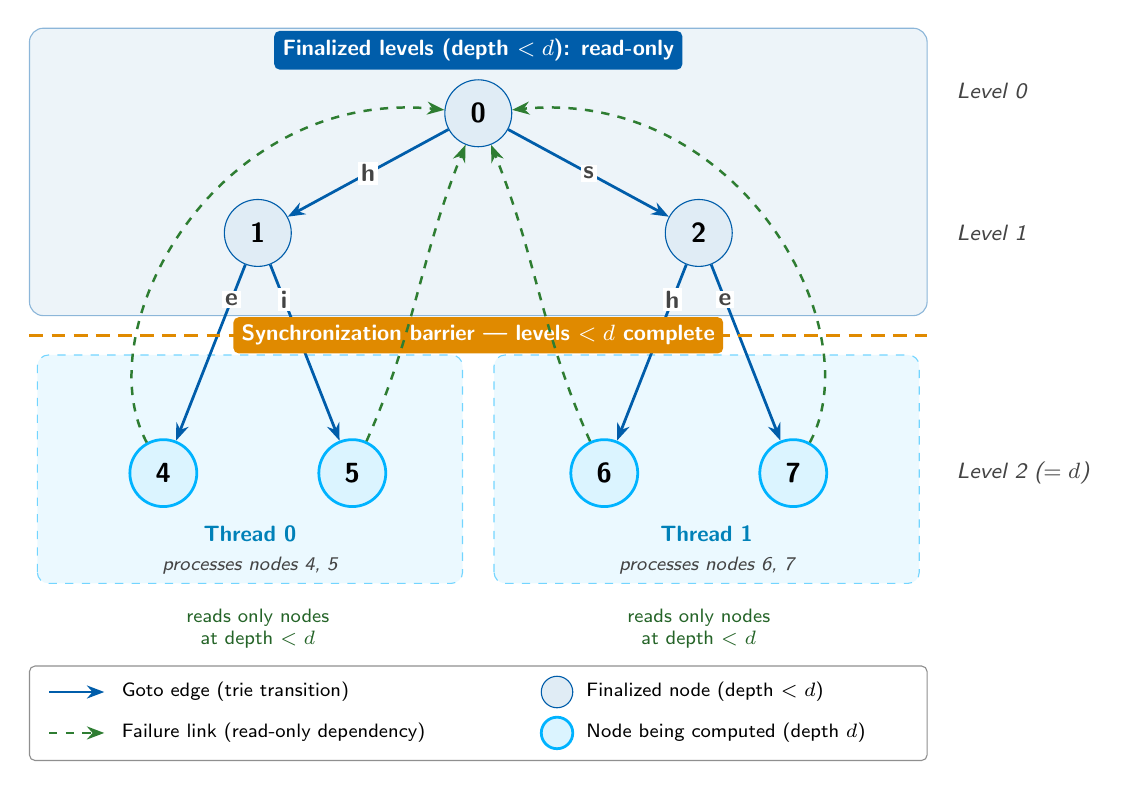
\begin{tikzpicture}[
    font=\small,
    >={Stealth[length=2.2mm]},
    state/.style={draw=inkgray, circle, minimum size=8.5mm, fill=gray!5,
                  font=\bfseries, inner sep=0pt},
    done/.style={state, draw=idpblue, fill=idpblue!12},
    active/.style={state, draw=idpcyan, line width=1.0pt, fill=idpcyan!14},
    goto/.style={->, line width=1.0pt, idpblue},
    fail/.style={->, dashed, line width=0.9pt, forestgreen},
    glabel/.style={font=\bfseries\small, text=inkgray, fill=white, inner sep=1pt},
    levtag/.style={font=\footnotesize\itshape, text=inkgray, anchor=west},
]

    % ============================================================
    %  ZONES (drawn on the background layer, behind everything)
    % ============================================================
    \begin{scope}[on background layer]
        % Finalized / read-only zone (levels < d)
        \fill[idpblue!7, rounded corners=5pt] (-5.7,1.55) rectangle (5.7,5.2);
        \draw[idpblue!45, rounded corners=5pt] (-5.7,1.55) rectangle (5.7,5.2);

        % Two thread bands inside the current (active) level
        \fill[idpcyan!8, rounded corners=4pt]  (-5.6,-1.85) rectangle (-0.2,1.05);
        \draw[idpcyan!55, dashed, rounded corners=4pt] (-5.6,-1.85) rectangle (-0.2,1.05);
        \fill[idpcyan!8, rounded corners=4pt]  (0.2,-1.85) rectangle (5.6,1.05);
        \draw[idpcyan!55, dashed, rounded corners=4pt] (0.2,-1.85) rectangle (5.6,1.05);
    \end{scope}

    % Zone captions
    \node[fill=idpblue, text=white, font=\footnotesize\bfseries, rounded corners=2pt,
          inner sep=3pt] at (0,4.92) {Finalized levels (depth $<d$): read-only};
    \node[font=\footnotesize\bfseries, text=idpcyan!72!black] at (-2.9,-1.22) {Thread 0};
    \node[font=\footnotesize\bfseries, text=idpcyan!72!black] at (2.9,-1.22)  {Thread 1};
    \node[font=\scriptsize\itshape, text=inkgray] at (-2.9,-1.62)
          {processes nodes 4, 5};
    \node[font=\scriptsize\itshape, text=inkgray] at (2.9,-1.62)
          {processes nodes 6, 7};

    % ============================================================
    %  NODES
    % ============================================================
    % Level 0
    \node[done] (r) at (0,4.12) {0};
    % Level 1
    \node[done] (n1) at (-2.8,2.6) {1};
    \node[done] (n2) at (2.8,2.6)  {2};
    % Level 2 (current level d) -- two nodes per thread
    \node[active] (c1) at (-4.0,-0.45) {4};
    \node[active] (c2) at (-1.6,-0.45) {5};
    \node[active] (c3) at (1.6,-0.45)  {6};
    \node[active] (c4) at (4.0,-0.45)  {7};

    % Right-hand level ruler
    \node[levtag] at (5.95,4.4)   {Level 0};
    \node[levtag] at (5.95,2.6)   {Level 1};
    \node[levtag] at (5.95,-0.45) {Level 2 ($=d$)};

    % ============================================================
    %  GOTO EDGES (trie transitions, solid)
    % ============================================================
    \draw[goto] (r) -- (n1) node[glabel, pos=0.5] {h};
    \draw[goto] (r) -- (n2) node[glabel, pos=0.5] {s};
    \draw[goto] (n1) -- (c1) node[glabel, pos=0.2] {e};
    \draw[goto] (n1) -- (c2) node[glabel, pos=0.2] {i};
    \draw[goto] (n2) -- (c3) node[glabel, pos=0.2] {h};
    \draw[goto] (n2) -- (c4) node[glabel, pos=0.2] {e};

    % ============================================================
    %  SYNCHRONIZATION BARRIER
    % ============================================================
    \draw[amber, line width=1.3pt, dash pattern=on 5pt off 3pt] (-5.7,1.3) -- (5.7,1.3);
    \node[fill=amber, text=white, font=\footnotesize\bfseries, rounded corners=2pt,
          inner sep=3pt] at (0,1.3) {Synchronization barrier --- levels $<d$ complete};

    % ============================================================
    %  FAILURE LINKS (dashed): every dependency points strictly UP,
    %  across the barrier, into the finalized read-only region.
    % ============================================================
    % outer links sweep wide, outside the level-1 nodes, then into the root
    \draw[fail] (c1) .. controls (-5.0,1.4) and (-3.3,4.45) .. (r);
    \draw[fail] (c4) .. controls (5.0,1.4)  and (3.3,4.45)  .. (r);
    % inner links rise straight up between the level-1 nodes
    \draw[fail] (c2) to[out=66,in=248]  (r);
    \draw[fail] (c3) to[out=114,in=292] (r);

    % Highlight the data-dependency rule on one representative node
    \node[font=\scriptsize, text=forestgreen!80!black, align=center, anchor=north]
        at (-2.8,-2.05)
        {reads only nodes\\ at depth $<d$};
    \node[font=\scriptsize, text=forestgreen!80!black, align=center, anchor=north]
        at (2.8,-2.05)
        {reads only nodes\\ at depth $<d$};

    % ============================================================
    %  LEGEND
    % ============================================================
    \begin{scope}[shift={(-5.7,-3.95)}]
        \draw[inkgray!60, fill=white, rounded corners=2pt] (0,-0.15) rectangle (11.4,1.05);
        \draw[goto] (0.25,0.72) -- (0.95,0.72);
        \node[anchor=west, font=\scriptsize] at (1.05,0.72) {Goto edge (trie transition)};
        \draw[fail] (0.25,0.2) -- (0.95,0.2);
        \node[anchor=west, font=\scriptsize] at (1.05,0.2) {Failure link (read-only dependency)};
        \node[done, minimum size=4mm, font=\tiny] at (6.7,0.72) {};
        \node[anchor=west, font=\scriptsize] at (6.95,0.72) {Finalized node (depth $<d$)};
        \node[active, minimum size=4mm, font=\tiny] at (6.7,0.2) {};
        \node[anchor=west, font=\scriptsize] at (6.95,0.2) {Node being computed (depth $d$)};
    \end{scope}

\end{tikzpicture}
\end{document}
